\section{Architektur und Komponenten}\label{sec:architektur-und-komponenten}

\textcolor{orange}{// TODO Hier noch Fehlerbehandlung behandeln? Wenn irgendwo ein Fehler passiert, wird der Testfall als fehlgeschlagen markiert und im Bericht vermerkt. Außerdem habe ich glaub ich am Anfang auch erwähnt, dass Fehlerhafte Testfälle nicht in die Metriken einfließen, oder? Das muss ich dann auch tatsächlich noch implmentieren, weil sie aktuell als falsch klassifiziert gezählt werden.}

Das Evaluationsframework ist modular aufgebaut und nutzt eine Pipeline-Architektur, um eine flexible und skalierbare Evaluierung zu ermöglichen, wie es in \hyperlink{FA02}{FA02} gefordert ist. Die Architektur ist in Abbildung~\ref{fig:evaluation-framework-architecture} dargestellt. Sie besteht aus mehreren Hauptkomponenten, die jeweils eine klar definierte Aufgabe erfüllen. Im Folgenden werden die Komponenten und ihr Zusammenspiel beschrieben.

\begin{figure}
    \centering
    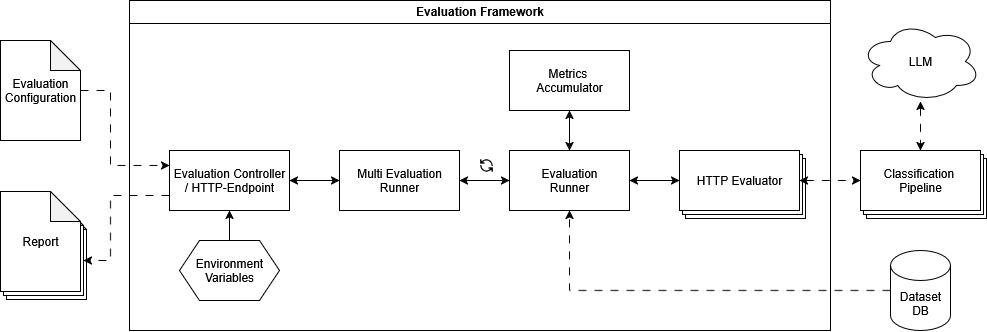
\includegraphics[width=\linewidth]{images/evaluation/evaluation-framework-architecture}
    \caption{Architektur des Evaluationsframeworks}
    \label{fig:evaluation-framework-architecture}
\end{figure}

\subsection*{Einstiegspunkte}

Das Framework bietet zwei Einstiegspunkte zur Ausführung einer Evaluierung:

\begin{itemize}
    \item \textbf{EvaluationController} als HTTP-Controller stellt REST-Endpunkte bereit, über die Evaluierungen gestartet werden können. Er akzeptiert eine YAML-Konfiguration und gibt die Ergebnisse entweder auf einmal als Markdown-Bericht oder als JSON-Stream zurück. Der Controller ermöglicht die Nutzung des Frameworks über die Weboberfläche, die in Kapitel \ref{sec:visualisierung-im-frontend} gezeigt wird, sowie über HTTP-APIs. Durch das Streamen der Ergebnisse können bereits abgeschlossene Testfälle sofort angezeigt werden, ohne auf das Ende der gesamten Evaluierung warten zu müssen.
    \item \textbf{EvaluationCommand} ist ein CLI-Befehl, der die Ausführung von Evaluierungen über die Kommandozeile erlaubt. Er liest eine YAML-Konfigurationsdatei ein, führt die Evaluierung aus und schreibt die Ergebnisse in eine Markdown-Datei. Dies eignet sich besonders für automatisierte Ausführungen, Continuous Integration oder die lokale Entwicklung.
\end{itemize}

Beide Einstiegspunkte akzeptieren die Konfiguration aus Kapitel \ref{sec:konfiguration-einer-evaluierung}, lösen ggf.\ Umgebungsvariablen auf und delegieren die Ausführung der Evaluation an den \texttt{MultiEvaluationRunner}.

\subsection*{Orchestrierung mit \texttt{MultiEvaluationRunner}}

Der \texttt{MultiEvaluationRunner} ist für die Orchestrierung der gesamten Evaluierung verantwortlich. Er verarbeitet die Konfiguration, die mehrere Modelle und Datensätze beschreibt, und koordiniert die sequenzielle Evaluierung aller konfigurierten Modelle. Für jedes Modell ruft der \texttt{MultiEvaluationRunner} den \texttt{EvaluationRunner} auf und übergibt diesem alle Informationen zur Ausführung der Evaluation eines einzelnen Modells.

Der \texttt{MultiEvaluationRunner} stellt zudem sicher, dass alle Modelle denselben Seed verwenden, um reproduzierbare Ergebnisse zu gewährleisten. Falls in der Konfiguration kein Seed angegeben wurde, wird an dieser Stelle einer erzeugt. Im Anschluss werden die Metadaten über die verwendeten Datensätze, Modelle, Endpunkte und den Seed gesammelt und als \texttt{MetadataReport} als Teil des Evaluationsberichts zurückgegeben. Die Teile des Berichts werden als \texttt{Flow} von Berichtartefakten zurückgegeben, wodurch eine streambasierte Verarbeitung ermöglicht wird. Welche Arten von Berichtartefakten es gibt, wird in kapitel \ref{sec:generierte-resultate} beschrieben.

\subsection*{Ausführung mit \texttt{EvaluationRunner}}

Der \texttt{EvaluationRunner} führt die Evaluierung für ein einzelnes Modell durch. Er lädt die Testfälle der angegebene Testdatensätze aus der Datenbank, führt die Klassifizierung für jeden Testfall aus und sammelt die Ergebnisse. Die Testfälle werden parallel verarbeitet, wobei die Anzahl der gleichzeitigen Ausführungen durch den Parameter \texttt{maxConcurrent} in der Konfiguration gesteuert wird. Dies ermöglicht es, Rate-Limits von \acp{LLM}-Diensten einzuhalten und die Auslastung der Ressourcen zu kontrollieren.

Für jeden Testfall delegiert der \texttt{EvaluationRunner} die eigentliche Klassifizierung an den \texttt{HttpEvaluator}. Anschließend vergleicht er die erwarteten mit den tatsächlichen Ergebnissen und berechnet die Klassifikationsmetriken wie \ac{TP}, \ac{FP}, \ac{FN} und \ac{TN}. Die Ergebnisse werden in \texttt{TestCaseReport}-Objekten zusammengefasst, als Teilergebnis zurückgegeben, und an den \texttt{MetricsAccumulator} weitergeleitet.

Der \texttt{EvaluationRunner} gibt die Ergebnisse ebenfalls als \texttt{Flow} zurück, wodurch eine frühzeitige Rückgabe von Teilergebnissen ermöglicht wird. Dies ist besonders vorteilhaft für die Live-Ansicht in der Weboberfläche, da Testfallergebnisse sofort nach ihrer Fertigstellung angezeigt werden können.

\subsection*{Klassifizierung mit \texttt{HttpEvaluator}}

Der \texttt{HttpEvaluator} ist für die Kommunikation mit dem Klassifizierungsendpunkt verantwortlich, der das in Kapitel \ref{sec:api-design} beschriebene Interface implementiert. Er nimmt das \ac{BPMN}-Modell aus dem aktuellen Testfall und die \texttt{llmProps} von dem aktuellen Modell aus der Konfiguration entgegen, baut einen HTTP-Request auf und sendet diesen an den konfigurierten Endpunkt. Nach erfolgreicher Klassifizierung extrahiert er die Liste der als kritisch identifizierten Aktivitäten aus der Antwort und gibt diese an den \texttt{EvaluationRunner} zurück.

\subsection*{Akkumulierung mit \texttt{MetricsAccumulator}}

Der \texttt{MetricsAccumulator} sammelt die Metriken aller Testfälle eines Modells und berechnet daraus aggregierte Werte. Er ist thread-sicher implementiert und kann gleichzeitig von mehreren parallelen Evaluierungen genutzt werden. Das ist wichtig, da der \texttt{EvaluationRunner} die Testfälle parallel ausführt und somit mehrere Threads gleichzeitig auf den \texttt{MetricsAccumulator} zugreifen können.

Nach Abschluss aller Testfälle erzeugt der \texttt{MetricsAccumulator} ein\break \texttt{EvaluationReportSummary}-Objekt, das alle Metriken für die Evaluation eines Modells über mehrere Testfälle hinweg enthält.

\subsection*{Zusammenfassung}

Die Architektur trennt Zuständigkeiten strikt:
\textt{MultiEvaluationRunner} koordiniert Modellläufe,
\textt{EvaluationRunner} verarbeitet Testfälle und sammelt Metriken,
\textt{HttpEvaluator} kommuniziert mit der Klassifizierungs-Pipeline,
\textt{MetricsAccumulator} aggregiert Ergebnisse pro Modell über mehrere Testfälle.
